\section{Functionnal Architecture}

\subsection{Introduction}
This constitutes the functional specifications of the project and allows us to have criteria
for the success of our project. \textbf{Figure~\ref{fig:requirement}} shows us the requirements
diagram that follows the \textit{SysML} standard for our system.

\subsection{Overview} % Not the right word I think

\begin{figure}[!ht]
    \begin{center}
        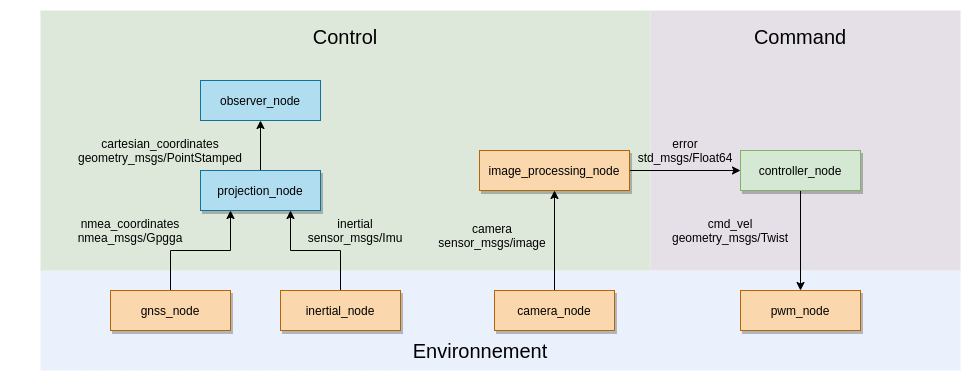
\includegraphics[scale=0.51]{Images/node_graph.png}
    \end{center}
    \caption{Functionnal Architecture of this project}
    \label{fig:requirement}
\end{figure}

\newpage